\section{Experiment 3: TransFuser with ensemble of three sets of weights trained from scratch}
\label{sec:exp3}
As pointed out in \cite{transfuser-pami},
agent performance of deep-learning methods can be sensitive to initial weight initialization.
We therefore train additional two sets of weights with different random seeds to obtain an ensemble of three sets of weights.

\subsection{Setup}
The training is performed identically to experiment 2,
and the evaluation identically to the previous two experiments.


\subsection{Results}

\begin{table}[]
    \centering
    \begin{tabular}{|c|c|}
        \hline
        \textbf{Metric} & \textbf{Result} \\ \hline
        Routes completed & 30 / 36 \\ \hline
        Driving score & 1.00\% \\ \hline
        Route completion & 3.63\% \\ \hline
        Infraction penalty & 0.308 \\ \hline
        Collisions with pedestrians & 0.0 \\ \hline
        Collisions with vehicles & 46.1 \\ \hline
        Collisions with layout & 29.98 \\ \hline
        Red light infractions & 0.73 \\ \hline
        Stop sign infractions & 0.0 \\ \hline
        Off-road infractions & 41.4 \\ \hline
        Route deviations & 0.0 \\ \hline
        Route timeouts & 2.19 \\ \hline
        Agent blocked & 19.74 \\ \hline
    \end{tabular}
    \caption{Results from experiment 3.}
    \label{tab:exp3:results}
\end{table}

In this experiment too, the model is evaluated using the Tesla Model 3.
We also see the expected failure to run the last 6 routes.
The driving score is very low, only 1\%,
due to a combination of a very low route completion and the infraction penalty.
Notably, the agent has a very high collision rate with vehicles and the scene geometry,
which causes it to get blocked in each of the 30 routes.
We also note an increase in the rate of red light infractions,
and a higher percentage of off-road driving.

The locations of the various infractions can be seen in \cref{fig:exp3:town02}.
In this experiment we observe fewer collisions in total,
but an increased count of the agent getting stuck.
Note that the agent gets stuck at places where it collides with either the scene geometry or other vehicles.

A video of this experiment can be found here: \url{https://youtu.be/ZREUj_nCAEA}.
In the video, the agents displays very poor performance.
It stops in the middle of the road,
and fails to drive further until the creeping mechanism kicks in,
after which it continues to drive slightly forward,
unfortunately in the middle of the road.
The car does stop at a red light,
but shortly after collides with an oncoming vehicle and gets permanently stuck.

\begin{figure}
    \centering
    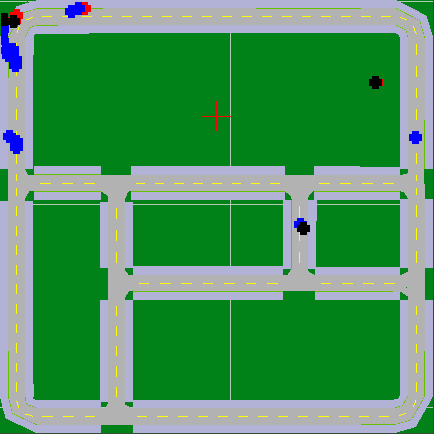
\includegraphics[width=0.5\textwidth]{chapters/4-experiments-results/figures/exp3-Town02.png}
    \caption{Infractions during experiment 3 on The town02 map.
    Red dots are collision with the scene geometry,
    and blue with other vehicles.
    The black dots mark places where the agent was permanently blocked.}
    \label{fig:exp3:town02}
\end{figure}


\subsection{Discussion}

This experiment demonstrated very bad driving capabilities.
The agent consistently collides with other vehicles or obstacles,
and thus gets stuck, unable to complete the route.
As a results, the route completion is drastically lower than in the other two experiments,
and the collision rates are far higher.
The increase in red-light and off-road infractions
also indicate a general decline in driving performance.

It is unclear why the agent performs so poorly.
Experiment 1 also uses an ensemble of agents and gives reasonable results,
and experiment 2 uses custom trained weights which also works reasonably well.
There are no apparent differences in the evaluation setup either which could explain these discrepancies.
There is however one possibility that should be investigated,
which is that the two other agents in our ensemble could perform very poorly individually,
and thus adversely affect the ensemble.
To evaluate these agents individually is left for future experiments.

As seen from \cref{fig:exp3:town02},
there are much fewer collisions in total than in the previous experiments.
This is due to the agent colliding once and getting stuck,
and thus doesn't get the chance to increase its collision count further.
The video reveals one possible failure mode and in general poor driving performance.
The agent did however stop at the red light.
In summary, this experiment did not produce an agent capable of driving well at all.
